
\documentclass{article}
\usepackage[utf8]{inputenc}
\usepackage{graphicx}
\usepackage{subcaption}
\usepackage{tikz} 
 \usetikzlibrary{arrows,automata,positioning,petri}
 
\title{Report on Labwork 9}
\author{TRAN Thi Hong Hanh}

\begin{document}

\maketitle
\section{Explain how you implement the labwork?}
\begin{itemize}
    \item Calculate histogram of input \textbf{grayscale} image. I used local histogram of a region in the image (GATHER) and then combine all of the region by a sum (REDUCTION) as described on the slide.
    \begin{verbatim}
__global__ void histogramGather(uchar3 *input, unsigned int **output,
                                                    int width, int height)
{
    unsigned int histoL[256] = {0};
    for (int i = 0; i < height; i++)
    {
        int j = input[blockIdx.x * height + i].x;
        histoL[j]++;
    }
    for (int i = 0; i < 256; i++)
    {
        output[blockIdx.x][i] = histoL[i];
    }
}

__global__ void histogramReduction(unsigned int **input, int *output,
                                                    int width, int height)
{
    // Dynamic shared memory size, allocated in host
    __shared__ unsigned int cache[256];

    // Cache the block content
    unsigned int localtid = threadIdx.x;
    cache[localtid] = 0;

    __syncthreads();

    // Reduction in cache
    for (int i = 0; i < width; i++)
    {
        cache[localtid] += input[i][localtid];
    }
    __syncthreads();

    // Only first thread writes back
    if (localtid == 0)
    {
        for (int i = 0; i < 256; i++)
        {
            output[i] = cache[i];
        }
    }
}        
    \end{verbatim}
    \item Equalize the histogram for that input image. I took advantage of grayscale in labwork 6, calculate the Cumulative distribution function (CDF), and equalize the histogram by increasing the global contrast and recalculate intensity. 
    \begin{verbatim}
__global__ void cdfCalculation(int *h, int pixelCount)
{
    int cdfMin = 0;
    int cdfCumul = 0;
    for (int i = 0; i < 256; i++)
    {
        if (cdfMin == 0)
        {
            cdfMin = h[i];
        }
        cdfCumul += h[i];
        h[i] = round((double)(cdfCumul - cdfMin) / (pixelCount - cdfMin) * 255.0);
    }
}

__global__ void equalization(uchar3 *input, int *h, uchar3 *output, 
                                                    int width, int height)
{
    int tidX = threadIdx.x + blockIdx.x * blockDim.x;
    if (tidX >= width)
        return;
    int tidY = threadIdx.y + blockIdx.y * blockDim.y;
    if (tidY >= height)
        return;
    int tid = tidX + tidY * width;

    unsigned char g = h[input[tid].x];
    output[tid].x = output[tid].y = output[tid].z = g;
}
    \end{verbatim}
    \item Command:
    \begin{verbatim}
        ./labwork 9 ../data/cloud_gray.jpg 
    \end{verbatim}
    \item Result:
    \begin{verbatim}
    USTH ICT Master 2019, Advanced Programming for HPC.
    Warming up...
    Starting labwork 9
    [ALGO ONLY] labwork 9 ellapsed 17.8ms
    Labwork 9 ellapsed 26.4ms
    \end{verbatim}
    \begin{figure}[h]
      \centering
      \begin{subfigure}{.45\textwidth}
        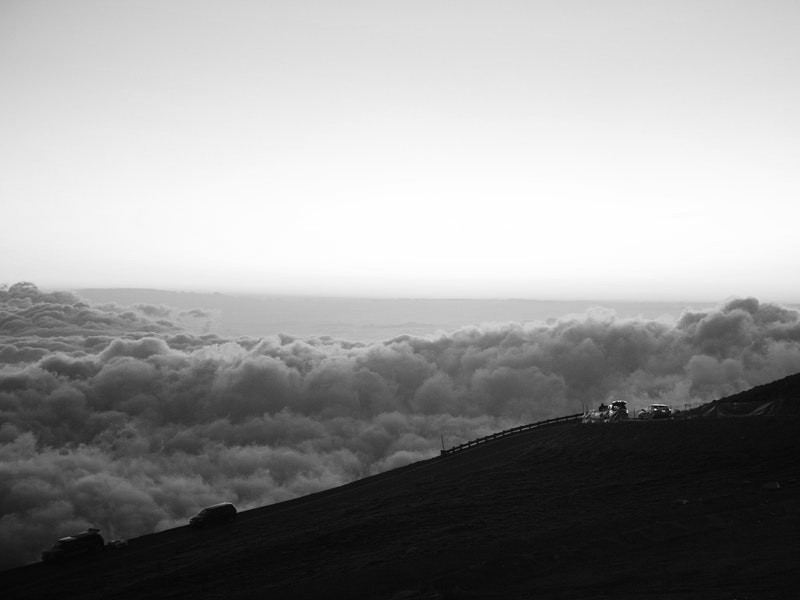
\includegraphics[width=\linewidth]{./result/cloud_gray.jpg}
        \caption{Original image}
      \end{subfigure}
      \hspace{1cm}
      \begin{subfigure}{.45\textwidth}
        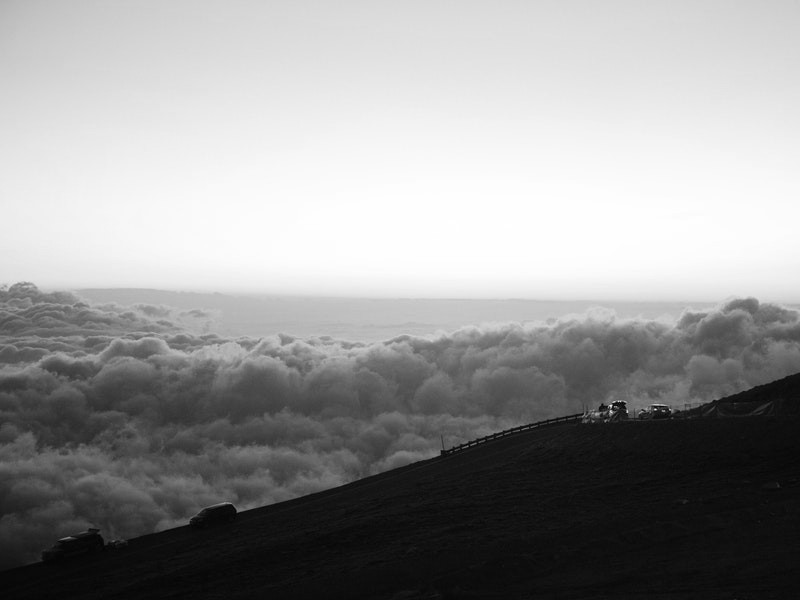
\includegraphics[width=\linewidth]{./result/labwork9-gpu-out.jpg}
        \caption{Equalized}
      \end{subfigure}
    \caption{The output image after histogram equalization have a slightly higher contrast compared to the original one.}
    \end{figure}
\end{itemize}


\end{document}

